%%%%%%%%%%%%%%%%%%%%%%%%%%%%%%%%%%%%%%%%%%%%%%%%%%%%%%%%%%%%%%%%%%%%%%%%
%%% ODE-based Latent Dynamics for LeWM-style JEPA World Models
%%% ECAI-style conference paper (ecai.cls)
%%%%%%%%%%%%%%%%%%%%%%%%%%%%%%%%%%%%%%%%%%%%%%%%%%%%%%%%%%%%%%%%%%%%%%%%
\documentclass{ecai}

\usepackage{amsmath,amssymb,amsthm}
\usepackage{booktabs}
\usepackage{graphicx}
\usepackage{hyperref}
\usepackage{cleveref}
\usepackage{enumitem}
\usepackage{multirow}
\usepackage{algorithm}
\usepackage{algpseudocode}

\newtheorem{definition}{Definition}
\newtheorem{remark}{Remark}

\newcommand{\method}{ODE-LeWM}
\newcommand{\LeWM}{LeWM}
\newcommand{\ODEWorld}{ODEWorld}

\begin{document}

\begin{frontmatter}

\title{Continuous-Time Latent Dynamics for JEPA World Models:\\
ODE Prediction in LeWorldModel}

\author[A]{\fnms{Boyi}~\snm{Li}}
\address[A]{Independent / AutoConference}

\begin{abstract}
Visual world models for control have progressed from pixel reconstruction
to joint-embedding prediction, enabling latent-space planning with
Cross-Entropy Method (CEM) and related MPC-style search.
Yet most JEPA-style stacks still advance latent state with a
\emph{discrete} autoregressive (AR) next-embedding map: one nonlinear
step must absorb an entire physical transition, with no explicit flow
along the planning interval and limited inductive bias toward temporal
coherence.
We propose \method{}, a visual world model whose latent dynamics are
\emph{continuous}: an action-conditioned neural ODE
$\mathrm{d}z/\mathrm{d}\tau = v_\theta(z,a)$, with one planning step
defined as fixed-step RK4 integration from $\tau{=}0$ to $\tau{=}1$.
Training keeps the standard JEPA next-embedding objective together with
SIGReg isotropic-Gaussian regularization; encoder, projectors, and the
CEM loop are unchanged so comparisons isolate continuous vs.\ discrete
latent evolution.
On the official PushT expert dataset with a fixed 1000-window subset
(seed~3072; train~901 / val~99), \method{} matches the discrete AR
baseline on val-tied CEM success (\textbf{5/93, $\approx$5.38\%}) while
achieving lower train and validation losses (0.234 / 0.506 vs.\
0.248 / 0.536).
We report limitations honestly: this subset is far below full-data
regimes that report high PushT success, and CEM is tied despite the
loss gain.
All numbers use the official Hugging Face release; no synthetic episodes
are used.

\end{abstract}

\end{frontmatter}

\section{Introduction}
\label{sec:intro}

\subsection{Motivation}
\label{sec:motivation}

World models that plan in a compact latent space enable fast
model-predictive control without decoding pixels at every step
\cite{ha2018worldmodels,hafner2019planet}.
Classical latent dynamics models often predict the next state with a
discrete transition (RNN, RSSM, or transformer block), then hand the
rollout to a planner such as CEM or MPPI.
Joint Embedding Predictive Architectures (JEPAs)
\cite{assran2023jepa} push the representation side further by
predicting future \emph{embeddings} rather than reconstructions,
avoiding a pixel decoder that can dominate compute and encourage
shortcut features.
Recent control-oriented JEPA stacks combine a ViT encoder trained from
scratch, an action-conditioned latent predictor, next-embedding MSE, and
SIGReg anti-collapse regularization~\cite{balestriero2025lejepa}, then
plan with CEM directly in latent space against a goal embedding.
Such systems can reach strong PushT success under full-data training,
but the predictor is typically still a discrete autoregressive block:
given context latents $z_t$ and action embeddings $a_t$, it directly
outputs $\hat z_{t+1}$.

Physical dynamics, however, are continuous in time.
A discrete next-step map must absorb the entire transition into a
single nonlinear layer, with no explicit notion of intermediate flow
along the planning interval.
That gap matters for temporal coherence, residual stability at
initialization, and---in principle---sharing structure across step
sizes when physical time is rescaled.
Recent continuous-time world models such as
\PriorODEWorld{}~\cite{liu2026odeworld} argue that latent velocity fields
$\mathrm{d}z/\mathrm{d}t = v_\theta(\cdot)$ better capture underlying
flow and support flexible temporal resolution.
Neural ODEs~\cite{chen2018neuralode} provide the standard tool for
parameterizing such fields and integrating them with classical
solvers.

We ask whether \emph{continuous} latent dynamics can serve as the
predictor inside an otherwise standard JEPA + SIGReg + CEM stack.
\method{} answers with an action-conditioned ODE velocity field and
RK4 integrate-to-next-step rule, reusing the same transformer capacity
as a discrete AR baseline under matched data and planning protocols.

\subsection{Contributions}
\label{sec:contributions}

\begin{enumerate}[leftmargin=*,itemsep=3pt]
\item \textbf{\method{} continuous latent predictor.}
We instantiate \method{} as an action-conditioned ODE inside a
JEPA-style visual world model:
$\mathrm{d}z/\mathrm{d}\tau = v_\theta(z,a)$, with one-step prediction
defined as classical RK4 integration over $\tau\in[0,1]$ (fixed
$N{=}4$ substeps), actions held constant on the interval, and a
zero-initialized linear velocity head for residual stability at
initialization.
The velocity backbone reuses the same ConditionalBlock / AdaLN-zero
transformer capacity as the discrete AR baseline
($\approx$18.07M parameters; +37{,}056 from the $v$-head).

\item \textbf{Matched 1k protocol on official data.}
We evaluate on the official Hugging Face PushT expert HDF5 with a
reproducible 1000-window split (seed~3072; 901 train / 99 val),
matching encoder, SIGReg ($\lambda{=}0.09$, $M{=}1024$), optimizer,
hardware batching (64$\times$accum~2), and CEM protocol between
discrete and ODE runs.
Indices are frozen and never regenerated between runs.

\item \textbf{Honest empirical findings.}
On this protocol, ODE lowers train/val loss relative to discrete AR
(0.234 / 0.506 vs.\ 0.248 / 0.536), while CEM success on the val-99
protocol is \textbf{tied} at 5/93~(5.38\%).
We explicitly contrast this with prior full-data PushT figures on the
order of $96\%$ success, and treat the 1k regime as a controlled
comparison rather than a claim of full-corpus performance.
No synthetic episodes are used.
\end{enumerate}

\paragraph{Why this matters.}
If continuous dynamics improve JEPA fit without destabilizing SIGReg or
CEM interfaces, visual world models can borrow ODE inductive bias without
abandoning latent MPC.
If they do not help planning under matched compute and data, that is
also useful: it suggests that predictor form is secondary to data scale
and planner configuration in the 1k regime.
Our results land in the middle---loss improves, CEM does not---and we
report both sides without overselling.

\paragraph{Scope.}
This paper is a controlled predictor comparison on PushT, not a
multi-environment bake-off or full-corpus training run.
Cube, Two-rooms, and Reacher remain future work
(\Cref{sec:limitations}).
We also do not convert or evaluate official Hugging Face pretrained
PushT weights under our val-99 protocol; that baseline remains future
work.

\section{Related Work}
\label{sec:related}

\subsection{JEPA, SIGReg, and \LeWM{}}
\label{sec:rel-jepa}

Joint Embedding Predictive Architectures learn predictive
representations by forecasting future embeddings rather than pixels
\cite{assran2023jepa}.
The JEPA objective is typically a distance between a predicted latent
and a target latent from a context encoder, often with stop-gradient
on the target path so the predictor cannot collapse by copying a
degenerate constant.
Video JEPA variants extend this idea to temporal sequences
\cite{bardes2024vjepa}, still avoiding reconstruction decoders that
can dominate loss and encourage shortcut visual features.
A recurring failure mode is \emph{representation collapse}: embeddings
that ignore inputs yet trivially satisfy a prediction objective.
SIGReg~\cite{balestriero2023sigreg} addresses collapse by pushing
projected embedding coordinates toward an isotropic Gaussian via a
sketched Epps--Pulley statistic, without requiring a stop-gradient
teacher network as in contrastive or BYOL-style recipes.

\LeWM{}~\cite{maes2026lewm} brings JEPA to end-to-end pixel world
models for control.
Its recipe is deliberately simple: a ViT encoder trained from scratch,
an action-conditioned predictor, MSE next-embedding loss, and SIGReg
with weight $\lambda{=}0.09$ and $M{=}1024$ projections.
Planning uses CEM in latent space against a goal embedding derived
from a future observation.
Reported PushT success under full-data training is high
($96{\pm}2.83\%$), which motivates careful protocol matching when
studying predictor variants on smaller subsets: a weak absolute CEM
score on 1k windows is expected and should not be confused with a
failed reproduction of the full recipe.
We adopt \LeWM{}'s official encoder, SIGReg recipe, projectors, and CEM
evaluator unchanged, so our study isolates predictor dynamics rather
than re-tuning the full stack.

\subsection{Continuous-time and ODE world models}
\label{sec:rel-ode}

Neural ODEs~\cite{chen2018neuralode} parameterize continuous
transformations via $\mathrm{d}z/\mathrm{d}t = v_\theta(z,t)$ and
backpropagate through ODE solvers.
This viewpoint has influenced continuous-depth networks, continuous
normalizing flows, and---more recently---world models that treat
latent evolution as a flow rather than a discrete jump.

\ODEWorld{}~\cite{liu2026odeworld} introduces Physical-Time Flow: a
continuous latent velocity field integrated by an ODE solver for video
and control, emphasizing dynamical representation structure beyond
discrete next-step prediction.
Our setting is narrower and deliberately comparable: we keep
\LeWM{}'s JEPA loss and planning loop, and redefine a single discrete
planning step as integrate $\tau{:}0\to 1$ under an
action-conditioned velocity field.
We do not claim the full Physical-Time Flow agenda (adaptive physical
time, multi-scale horizons, or ODEWorld's broader architecture);
instead we ask whether the ODE inductive bias alone helps under a
matched \LeWM{} protocol.

\subsection{Discrete AR vs.\ continuous latent dynamics}
\label{sec:rel-disc-cont}

Discrete autoregressive predictors map $(z_t,a_t)\mapsto\hat z_{t+1}$
in one shot.
They are efficient at inference (one forward pass per step) and match
the discrete action schedule used by CEM rollouts.
Continuous predictors instead learn $v_\theta$ and obtain
$\hat z_{t+1}$ by numerical integration.
This costs more compute per step (RK4 with $N{=}4$ evaluates the
velocity field four times per substep interval, sixteen times over
$\tau{:}0\to1$ with $N{=}4$), but exposes intermediate states along
the interval and encourages residual updates ($z(1)\approx z(0)$ when
$v\approx 0$).
Our experiments quantify both sides: loss and CEM on a fixed split,
plus wall-clock CEM cost on the same hardware.

\subsection{Latent MPC and CEM planning}
\label{sec:rel-cem}

Model-based RL and planning systems often learn latent dynamics and
optimize action sequences by shooting
\cite{chua2018pets,hafner2019planet}.
Cross-entropy method (CEM) samples candidate action sequences, rolls
out the learned dynamics, ranks by a goal-conditioned cost, and
refits a sampling distribution around elite samples.
\LeWM{} uses this interface with a latent goal embedding derived from
a future observation at a fixed goal offset.

We use the official \LeWM{} CEM evaluator on a fixed validation window
set so discrete and ODE predictors share the same starts and
feasibility filter (\Cref{sec:setup}).
Earlier probes on random full-dataset starts are discarded as
protocol-mismatched; all planning claims in this paper use the
val-99 / 93-feasible protocol tied to \texttt{validate/loss}.

\subsection{Positioning summary}
\label{sec:rel-position}

Relative to prior work, \method{} is intentionally conservative:
\begin{itemize}[leftmargin=*,itemsep=2pt]
\item vs.\ \LeWM{}: same JEPA + SIGReg + CEM stack; only the predictor
map changes from discrete AR to RK4-integrated $v_\theta$.
\item vs.\ \ODEWorld{}: we borrow the continuous-velocity idea, but do
not adopt Physical-Time Flow, adaptive physical time, or ODEWorld's
full training recipe.
\item vs.\ classical Neural ODEs: we integrate on a fixed normalized
interval $\tau\in[0,1]$ per planning step, with piecewise-constant
actions, rather than learning an unrestricted continuous-time policy.
\end{itemize}
This positioning keeps comparisons fair on official PushT windows and
makes negative or tied CEM results interpretable rather than confounded
by simultaneous encoder or planner changes.

\section{Method}
\label{sec:method}

We keep the \LeWM{} JEPA backbone~\cite{maes2026lewm} and replace only
the discrete AR predictor with an ODE velocity field.
Notation follows the official implementation (history length $H{=}3$,
embedding dimension $D{=}192$).

\subsection{Encoder and action embedding}
\label{sec:encoder}

Let $x_{t-H+1:t}$ be a stack of RGB observations (resolution
$224{\times}224$).
A ViT-tiny encoder $f_\phi$ (patch size 14, trained from scratch)
maps each frame to a CLS token; an MLP projector $p$ yields latents
\begin{equation}
  z_t \;=\; p\bigl(f_\phi(x_t)\bigr) \in \mathbb{R}^{D}.
  \label{eq:encode}
\end{equation}
Actions $u_t$ are mapped by an embedder $e_\psi$ to
$a_t = e_\psi(u_t)\in\mathbb{R}^{D}$.
Context tensors for one prediction step are
$Z = (z_{t-H+1},\ldots,z_t)$ and $A = (a_{t-H+1},\ldots,a_t)$.

\subsection{Discrete baseline predictor}
\label{sec:ar}

The official \LeWM{} predictor is an action-conditioned transformer
(ConditionalBlock / AdaLN-zero) of depth 6, 16 heads, width $D$:
\begin{equation}
  \hat Z_{t+1}
  \;=\;
  g^{\mathrm{AR}}_\theta(Z, A),
  \label{eq:ar}
\end{equation}
interpreted as the next latent window (same shape as $Z$).
A prediction head MLP $q$ is applied after the predictor for the MSE
term (unchanged in our ODE variant).

\subsection{ODE predictor}
\label{sec:ode}

We reinterpret the same transformer capacity as a
\textbf{velocity field} $v_\theta$, with a zero-initialized linear
head $W_v$ (adds $D^2{+}D{=}37{,}056$ parameters):
\begin{equation}
  v_\theta(z, a)
  \;=\;
  W_v\,\mathrm{TF}_\theta\bigl(z + \mathrm{PE},\, a\bigr),
  \label{eq:velocity}
\end{equation}
where $\mathrm{PE}$ is a learnable positional embedding over the
history axis and actions $a$ condition AdaLN as in the AR baseline.
Latent dynamics on a normalized step interval $\tau\in[0,1]$ are
\begin{equation}
  \frac{\mathrm{d}z}{\mathrm{d}\tau}
  \;=\;
  v_\theta\bigl(z(\tau),\, a\bigr),
  \qquad
  z(0) = Z,
  \label{eq:ode}
\end{equation}
with $a$ \emph{held fixed} over the interval (piecewise-constant
action, matching one CEM planning step).
\textbf{One-step prediction} is the solution at $\tau{=}1$:
\begin{equation}
  \hat Z_{t+1}
  \;=\;
  z(1)
  \;=\;
  Z + \int_{0}^{1} v_\theta\bigl(z(\tau),\, a\bigr)\, \mathrm{d}\tau.
  \label{eq:onestep}
\end{equation}
We approximate the integral with fixed-step classical RK4 using
$N{=}4$ substeps ($h{=}1/N$):
\begin{align}
  k_1 &= v_\theta(z,a), \nonumber\\
  k_2 &= v_\theta(z + \tfrac{h}{2}k_1,\, a), \nonumber\\
  k_3 &= v_\theta(z + \tfrac{h}{2}k_2,\, a), \nonumber\\
  k_4 &= v_\theta(z + h\,k_3,\, a), \nonumber\\
  z &\leftarrow z + \tfrac{h}{6}(k_1 + 2k_2 + 2k_3 + k_4).
  \label{eq:rk4}
\end{align}
Zero-init of $W_v$ yields $v\approx 0$ at initialization, hence
$z(1)\approx z(0)$ (stable residual ODE).

\subsection{Training objective (SIGReg + prediction)}
\label{sec:loss}

Following \LeWM{}, the total loss is
\begin{equation}
  \mathcal{L}
  \;=\;
  \mathcal{L}_{\mathrm{pred}}
  \;+\;
  \lambda\,\mathcal{L}_{\mathrm{SIGReg}},
  \qquad
  \lambda = 0.09,
  \label{eq:loss}
\end{equation}
where $\mathcal{L}_{\mathrm{pred}}$ is MSE between projected
predictions and target embeddings (stop-grad on targets), and
$\mathcal{L}_{\mathrm{SIGReg}}$ is the sketched Epps--Pulley statistic
over $M{=}1024$ random projections and 17 quadrature knots
\cite{balestriero2023sigreg,maes2026lewm}.
Only the predictor internals differ between discrete and ODE runs;
encoder, projectors, SIGReg, and optimizer are shared.

\subsection{Planning with CEM}
\label{sec:cem}

At evaluation, Cross-Entropy Method (CEM) samples action sequences,
rolls out the predictor in latent space from encoded pixels, and
selects the plan minimizing distance to a goal embedding (official
PushT CEM config).
For the ODE model, each rollout step applies
\eqref{eq:onestep}--\eqref{eq:rk4} instead of \eqref{eq:ar}.

\section{Experiments}
\label{sec:exp}

\subsection{Setup}
\label{sec:setup}

\paragraph{Data.}
We use only the official Hugging Face PushT expert release
(\texttt{quentinll/lewm-pusht}, HDF5).
A reproducible subset of \textbf{1000} windows is drawn with seed
\textbf{3072} and split by \texttt{spt.random\_split([0.9, 0.1])} into
\textbf{901} train / \textbf{99} validation windows
(indices frozen; never regenerated between runs).
Of the 99 val windows, \textbf{93} remain feasible under
\texttt{goal\_offset=25} for CEM (6 dropped).

\paragraph{Models and compute.}
Both predictors use ViT-tiny, history 3, $D{=}192$, SIGReg
$\lambda{=}0.09$, AdamW lr $5{\times}10^{-5}$, weight decay
$10^{-3}$, grad clip 1.0, bf16, 100 epochs, frameskip 5.
Hardware: RTX~4060 Laptop (8\,GiB); batch 64 with gradient
accumulation 2 (effective 128); \texttt{num\_workers=0}.
Parameter counts: discrete AR \textbf{18,034,478}; ODE
\textbf{18,071,534} (+37,056 from $v$-head).

\begin{table}[t]
\centering
\caption{Experimental setup (PushT 1k subset).}
\label{tab:setup}
\begin{tabular}{lc}
\toprule
Item & Value \\
\midrule
Dataset & Official HF PushT expert HDF5 \\
Subset / seed & 1000 windows / 3072 \\
Train / val & 901 / 99 \\
CEM eval set & val-99 $\to$ 93 feasible \\
Encoder & ViT-tiny, patch 14, $224^2$, scratch \\
SIGReg & $\lambda{=}0.09$, $M{=}1024$, knots 17 \\
ODE solver & RK4, $N{=}4$, $\tau{:}0\to1$ \\
Params (ODE) & 18,071,534 ($\approx$18.07M) \\
Train & 100 epochs, AdamW $5{\times}10^{-5}$ \\
Effective batch & 128 (64$\times$accum~2) \\
\bottomrule
\end{tabular}
\end{table}

\subsection{Results}
\label{sec:results}

\begin{table}[t]
\centering
\caption{PushT 1k$\times$100ep: loss and CEM (same split).
Paper PushT success is under full-data training, shown for context only.}
\label{tab:results}
\begin{tabular}{lcccc}
\toprule
Method & Params & fit/loss & val/loss & CEM val-99 \\
\midrule
Discrete AR (\LeWM{}) & 18.03M & 0.248 & 0.536 & 5/93 (5.38\%) \\
ODE RK4 0$\to$1 (ours) & 18.07M & \textbf{0.234} & \textbf{0.506} & 5/93 (5.38\%) \\
\midrule
\LeWM{} paper (full data) & $\sim$15M & --- & --- & $96{\pm}2.83$\%$^\dagger$ \\
\bottomrule
\multicolumn{5}{l}{\footnotesize $^\dagger$Reported PushT success; not comparable to our 1k protocol.} \\
\end{tabular}
\end{table}

\begin{figure}[t]
\centering
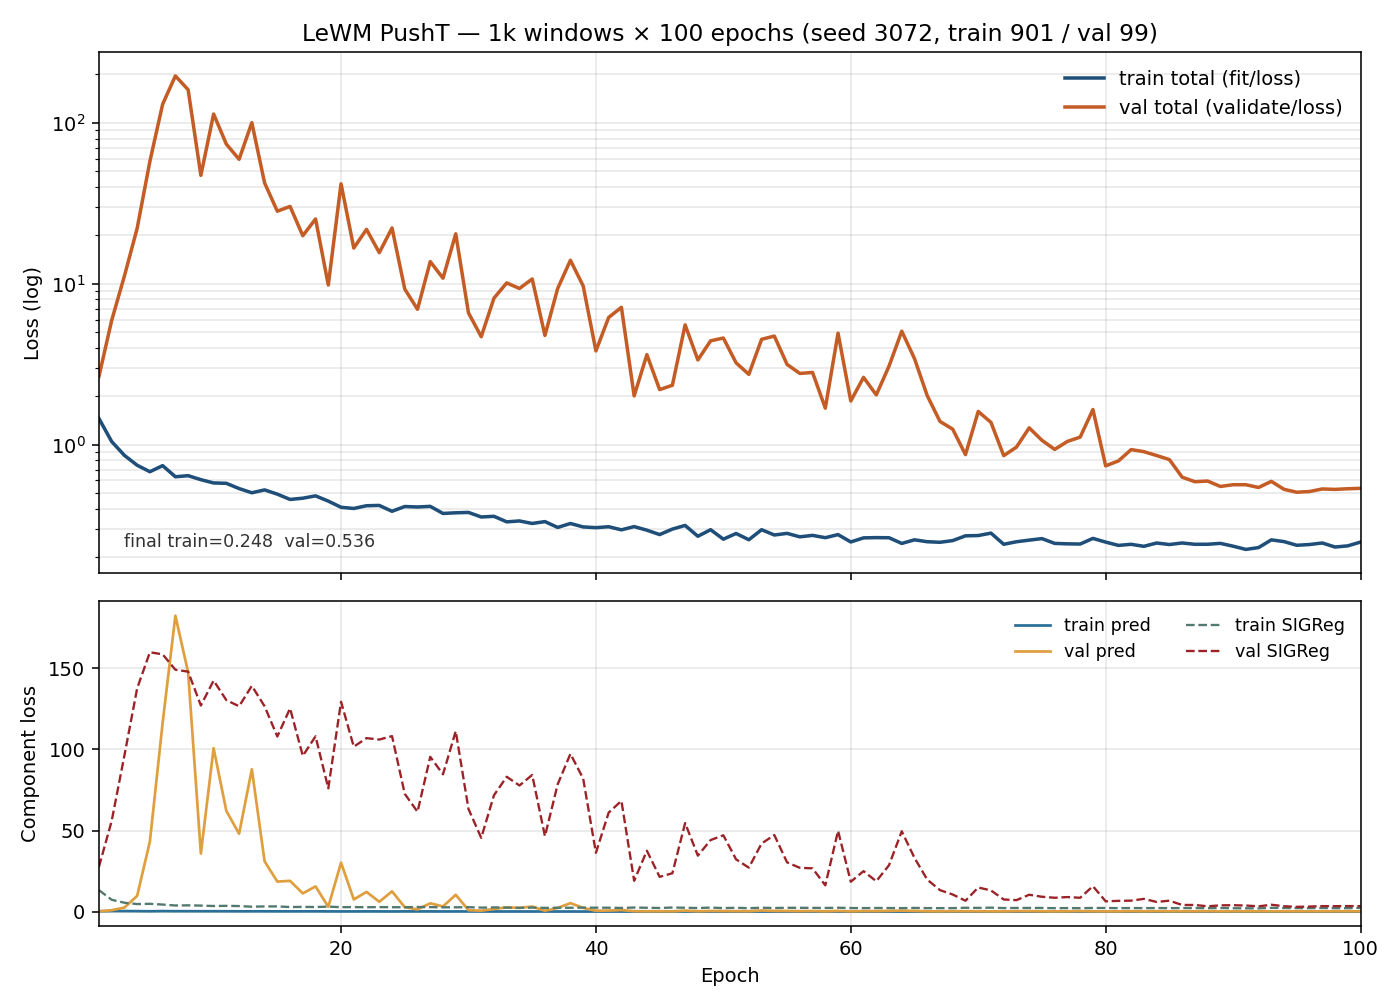
\includegraphics[width=0.48\linewidth]{figs/lewm_train_loss.png}%
\hfill
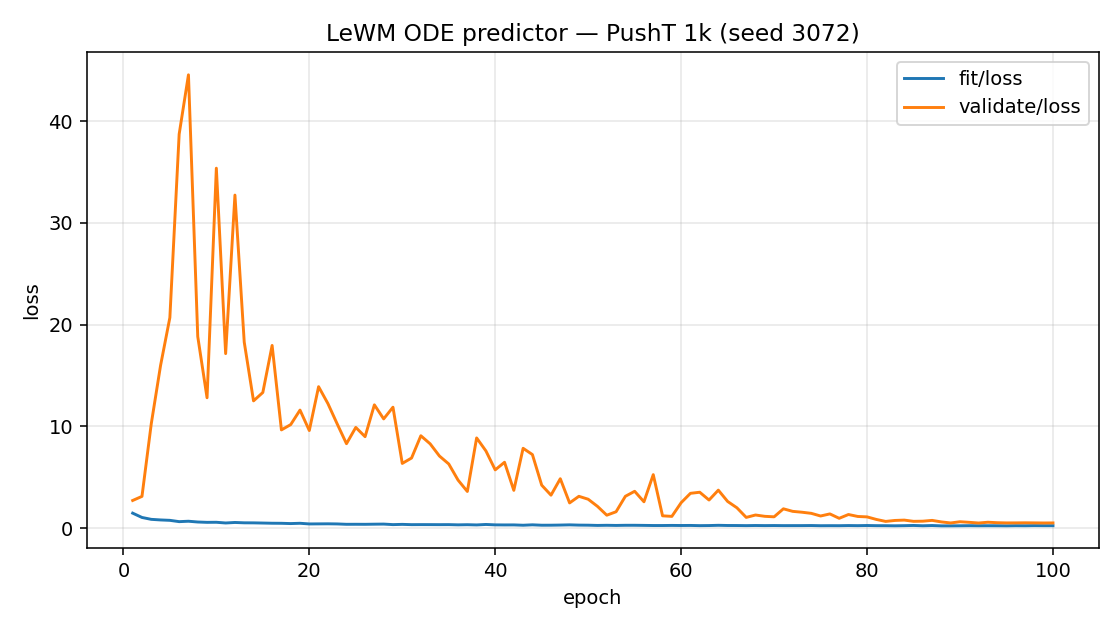
\includegraphics[width=0.48\linewidth]{figs/lewm_ode_train_loss.png}
\caption{Training curves on the fixed 1k split (left: discrete AR;
right: ODE predictor). ODE converges to lower fit/val loss.}
\label{fig:curves}
\end{figure}

Table~\ref{tab:results} summarizes the matched comparison.
The ODE predictor improves fit/loss (0.234 vs.\ 0.248) and val/loss
(0.506 vs.\ 0.536); final val prediction / SIGReg terms are
approximately 0.220 / 3.17.
CEM success is identical: \textbf{5 successes out of 93} feasible
val starts ($\approx$5.38\%).
ODE CEM wall-clock is substantially higher ($\approx$82\,min vs.\
$\approx$8\,min for discrete on the same machine) because each
rollout step runs four RK4 stages.

\paragraph{Protocol note.}
Earlier CEM probes on random full-dataset starts (e.g.\ 0/10) are
\emph{not} val-tied and are discarded; all claims here use the
val-99 / 93-feasible protocol shared with \texttt{validate/loss}.

\subsection{Limitations}
\label{sec:limitations}

\begin{itemize}[leftmargin=*,itemsep=2pt]
\item \textbf{1k subset.} Results are on 1000 windows, not the full
PushT expert corpus. Paper-scale $\approx$96\% success is out of
scope for this study.
\item \textbf{CEM tied.} Lower loss does not yield higher CEM success
under this budget; planning may be bottlenecked by data scale, CEM
hyperparameters, or goal-offset feasibility rather than predictor
form.
\item \textbf{Single environment.} Only PushT is evaluated; Cube,
Two-rooms, and Reacher remain future work.
\item \textbf{Fixed solver.} We use RK4 with $N{=}4$ and no adaptive
stepping; broader ODE solvers and multi-step $\tau$ schedules are
unexplored.
\end{itemize}

\section{Conclusion}
\label{sec:conclusion}

We presented a minimal continuous-time drop-in for \LeWM{}-style JEPA
world models: an action-conditioned ODE predictor whose one-step map
is RK4 integration from $\tau{=}0$ to $\tau{=}1$.
On official PushT data with a fixed 1k-window split, the ODE model
matches discrete AR CEM success (5/93) while reducing train and
validation loss.
The result supports continuous latent dynamics as a viable predictor
inductive bias for planning JEPA models, but---honestly---does not
yet improve CEM under the 1k regime, nor close the gap to
paper-scale PushT performance.
Natural next steps are full-dataset training, multi-environment CEM,
and stronger continuous-time formulations in the spirit of
\ODEWorld{}~\cite{liu2026odeworld}.


\bibliography{refs}

\end{document}
